%%%%%%%%%%%%%%%%%%%%%%%%%%%%%%%%%%%%%%%%%%%%%%%%%%%%%%%%%%%%%%%%%%%%%%%
%%%                           System Description
%%%%%%%%%%%%%%%%%%%%%%%%%%%%%%%%%%%%%%%%%%%%%%%%%%%%%%%%%%%%%%%%%%%%%%




\chapter{Evaluation}

The goal was to confirm whether our game could improve the correctness of identifying phishing emails with a statistically significant result and understand common patterns found among users who fall for phishing attacks.

\section{Test Design}
Since we want to understand the improvement after the user plays the game, we present each user with pre-survey and post-survey questions. Both surveys contain the same email users have to classify as phishing, legitimate, or need more information (maybe phishing). In addition, we ask the user to provide an optional field to provide feedback on the choice they made.

We curated a list of 12 emails with eight phishing emails and four legitimate emails. We replicated emails from Netflix, a common service used by many individuals. In addition to emails from Netflix, we also had an email from a "co-worker." The context of the email was pre narrated in the survey question. Using emails from a domain different than PayPal allowed us to verify that our game works across different domains.

Emails for our evaluation were hand-picked from the most common phishing emails we found during our research (commonly listed in different articles, multiple occurrences in Google search). The emails include suspicious account warnings such as payment failure, login attempts, suspicious logins, account cancellation, et cetera, and some common too good to be true emails such as free Netflix. We present these emails to the user in a Gmail clone \footnote{\url{https://github.com/codermother/Gmail-Clone}}. Figure \ref{fig:evaluation_site} shows the Gmail clone site with some emails. Although the site looks visually similar to Gmail, it has limited functionality and only allows users to click on "Inbox."

\begin{figure}[!ht]
    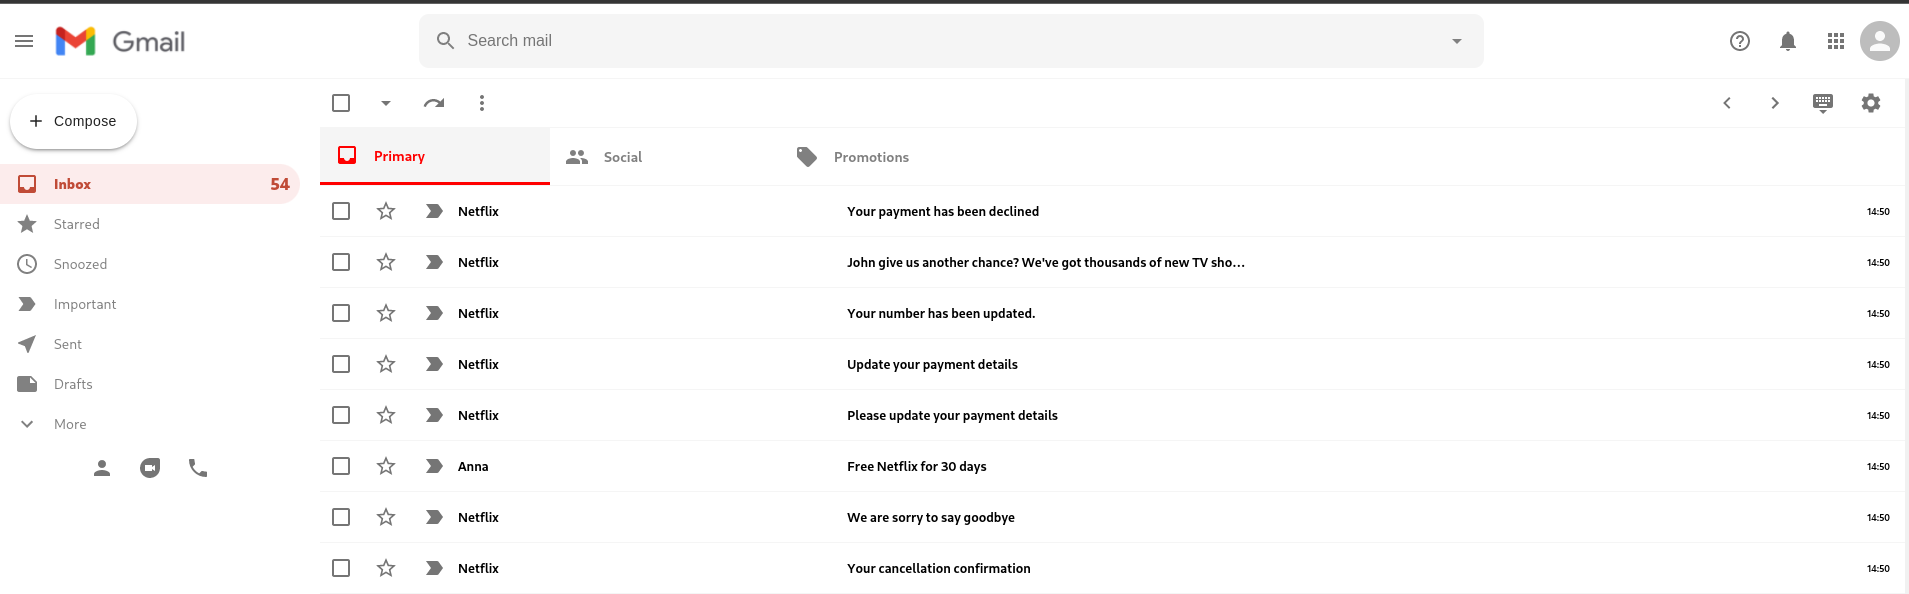
\includegraphics[width=\textwidth]{section3/evaluation_site.png}
    \caption{The Gmail clone used during evaluation with list of custom emails}
    \label{fig:evaluation_site}
\end{figure}

To evaluate engagement, we ask the participants various 5-point Likert scale ration questions in the post survey. These questions were derived from "Smells Phishy?"\cite{smels_phishy}.


\section{Methodology}
\textbf{Participants}: We distributed the evaluation (along with the game) primarily through email. In addition, we had a group meeting where players completed the survey in person. In total, 13 people attempted the game. However, only 11 participants completed both the presurvey and post-survey. Therefore, we will not consider the data for the two people that did not complete the post-survey. There were four female and seven male participants. All the participants were between 20 and 40, with seven participants in the range 20-30 and 4 participants in the range 30-40. Most of our participants were currently university students, and except for one, all were either enrolled or had a previous background in computer science. The one participant that did not have a Computer Science background had a degree in Biology.

\textbf{Sessions} : All the participants had a single flow for the study.
\begin{enumerate}
    \setlength{\itemsep}{0pt}
    \setlength{\parskip}{0pt}
    \setlength{\topsep}{0pt}
    \item Complete the pre-survey and obtain the passcode for the game. The pre-survey contains some general demographic questions and email classification questions.
    \item  Play the game. We provide the post-survey link after the player completes the game. Players can restart the game from the current week if they fail to complete it in a single try.
    \item Complete the post-survey. The post-survey contains the same set of email classification questions. In addition, it contains questions regarding game engagement.
\end{enumerate}

\textbf{Data Collection}: In addition to the data collected through pre-survey and post-survey, we keep track of all activity of players in the game. This log helps us verify that players played the game in the order we want and can be used to improve future iterations of the game.

\section{Results}
\subsection{Pre-Survey}
The pre-survey responses provided the participant's pre-existing knowledge of phishing scams. Participants chose one of three options (as discussed above in test design): Phishing, Legitimate, and Need more information (maybe phishing). To understand user thought behind their selection, we provide an optional text area to explain the user choice.

Each user option is classified as below:

\begin{enumerate}
    \setlength{\itemsep}{0pt}
    \setlength{\parskip}{0pt}
    \setlength{\topsep}{0pt}
    \item \textbf{True Positive}: The user correctly classified the email as phishing.
    \item \textbf{True Negative}: The user correctly classified the email as legitimate.
    \item \textbf{False Positive}: The user incorrectly classified legitimate emails as phishing emails.
    \item \textbf{False Negative}: The user incorrectly classified phishing emails as legitimate emails.
\end{enumerate}

Since participants could mark emails, they are not confident with as "Maybe," we analyze our data in two separate ways, first by neglecting emails marked as "Maybe," and second by including all the results. On average, participants marked 17.41\% of questions as "Maybe" in our presurvey. Since marking an email as "Maybe" shows caution and does not engage the user, we treat these results as "Marked phishing." Hence, phishing emails marked as "Maybe" are classified as "True Positive," and legitimate emails marked as "Maybe" are classified as "False Positive."

Table \ref{tab:pre_survey_responses} shows the average performance (in percent) of each user when we ignore questions marked as "Maybe" and Table \ref{tab:pre_survey_responses_all} show the average perfomance (in percent) when we include all the result and treat "Maybe" as phishing.

\begin{table}[!ht]
    \begin{center}

        \begin{tabular}{c | c c}
            Actual              & \multicolumn{2}{c}{User response}                       \\
                                & \textbf{Phishing}                 & \textbf{Legitimate} \\
            \textbf{Phishing}   & 63\%                              & 37\%                \\
            \textbf{Legitimate} & 7\%                               & 93\%                \\
        \end{tabular}
        \caption[Average performance in pre-survey (I)]{Average performance in pre-survey when we ignore emails marked as "Maybe"}
        \label{tab:pre_survey_responses}
    \end{center}
\end{table}

\begin{table}[!ht]
    \begin{center}

        \begin{tabular}{c | c c}
            Actual              & \multicolumn{2}{c}{User response}                       \\
                                & \textbf{Phishing}                 & \textbf{Legitimate} \\
            \textbf{Phishing}   & 74\%                              & 26\%                \\
            \textbf{Legitimate} & 23\%                              & 77\%                \\
        \end{tabular}
        \caption[Average performance in pre-survey (II)]{Average performance in pre-survey when we include all the results and treat "Maybe" as marked phishing}
        \label{tab:pre_survey_responses_all}
    \end{center}
\end{table}

Based on these result (Table \ref{tab:pre_survey_responses} and \ref{tab:pre_survey_responses_all}), we assume participants have some  beforehand knowledge about phishing emails. However, we can also see some confusion with legitimate vs. phishing emails based on the number of emails marked as "Maybe" (17.41\%)

We manually reviewed the user text responses to understand why they made each decision. We noticed similar thought processes in many of the participants:

\begin{enumerate}
    \item Participants who missed phishing emails were more suspicious of the content of the email. For example, some participants thought organizations do not send emails regarding common account information/errors such as subscription cancellation, number update, etc. Account update emails are commonly sent to the account holder by existing popular services.
    \item Only a couple of participants actively looked at technical details such as the link and the sender. Since participants focused more on the context of the email, any email that asked or put some personal context in the email was marked as potentially phishing or phishing.
\end{enumerate}

\subsection{Game}
Users start the game after the pre-survey. Since we distributed the game through email, we need to verify that the user completed the survey before attempting the game. Therefore, we lock the game with a passcode, provided at the end of the pre-survey.

Participants took a little over 25 minutes to complete the game. The fastest recorded time was 18 minutes, and the longest was 43 minutes. We noticed that participants took the longest in Week 3, where they had to play around with different domains. Table \ref{tab:game_time} shows the average time user took for each week.

\begin{table}[!ht]
    \centering
    \begin{tabular}{r r r r }
        \hline
        \textbf{Week} & \textbf{Average Time} & \textbf{Fastest Time} & \textbf{Slowest Time} \\
        1             & 2.27                  & 1.77                  & 2.80                  \\
        2             & 5.18                  & 4.18                  & 6.73                  \\
        3             & 10.54                 & 2.11                  & 18.18                 \\
        4             & 8.54                  & 4.00                  & 23.43                 \\
        \hline
    \end{tabular}
    \caption{Average time user took for each week (in minutes)}
    \label{tab:game_time}
\end{table}

Participants quickly figured out spelling and grammar errors in Week 1 and did not have trouble understanding different link hiding techniques in Week 2. However, many participants had to redo Week 3 as they could not find good domains to try. Some participants tried domains that had no connection with PayPal, such as "starbucks.com," "fredmeyer.com," and "youtube.org." However, participants successfully figured out that purchasing similar domains provided better efficiency. Table \ref{tab:marketplace_domains} shows different domains used in the game.

\begin{table}[!ht]
    \centering
    \begin{tabular}{l c  }
        \hline
        \textbf{Domains}       & \textbf{Number of used} \\
        paypal.org             & 8                       \\
        paypai.com             & 8                       \\
        paypal.co              & 4                       \\
        paypal.nl              & 1                       \\
        info-paypal.com        & 1                       \\
        youtube.org            & 1                       \\
        paypalsupport.com      & 1                       \\
        paypayl-info-gmail.com & 1                       \\
        paypal-paypal.com      & 1                       \\
        billingpal.com         & 1                       \\
        paypay-hotmail.com     & 1                       \\
        paypal.gov             & 1                       \\
        paypal.cm              & 1                       \\
        startbucks.com         & 1                       \\
        fredmeyer.com          & 1                       \\
        \hline
    \end{tabular}
    \caption{Different domains purchased in the marketplace in game}
    \label{tab:marketplace_domains}
\end{table}

Although most participants chose domains with the alternate ending as suggested by the game (when they enter paypal.com), some users were creative and figured our purchasing paypaI.com (with i) would make it look visually similar and be more efficient. We did not consider visual similarity in this iteration, and it can be something to consider in future iterations.

A few participants had a problem with spoofing, but generally, participants quickly understood spoofing and used efficient email addresses. Table \ref{tab:spoofing_emails} shows different emails used by participants during spoofing. Participants used efficient domains (paypal.com) with commonly seen names such as accounts, contact, support, etc.

\begin{table}
    \centering
    \begin{tabular}{l}
        \hline
        \textbf{Emails used by participants} \\
        \hline
        accounts@paypal.com                  \\
        admin@paypal.com                     \\
        alert@paypal.com                     \\
        ben@paypal.com                       \\
        contact@paypal.com                   \\
        customerservice@paypal.com           \\
        paypal@gmail.com                     \\
        paypalsecurity@pp.com                \\
        paypalsupport@paypal.com             \\
        security@paypal.com                  \\
        support@paypal.com                   \\
        \hline
    \end{tabular}
    \caption{Some spoofing emails used by participants}
    \label{tab:spoofing_emails}
\end{table}

Overall, we believe participants were able to play the game smoothly and complete all the game objectives without any hiccups. Furthermore, based on the game logs, players explored all the goals in the game (even though most players had to play the game at least a couple of times).

\subsection{Post-Survey}
The post-survey responses give us an idea of our game's effectiveness by allowing us to compare the before and after game scores. In addition to classifying the emails, we ask the participants 5-point Likert scale questions.

Like pre-evaluation, we evaluate the user performance on two different scales, one without emails marked as "Maybe" and one with all the emails. We repeat the same process for the second part (with maybe) as done in the presurvey. Emails marked as "Maybe" are treated as "Phishing."

After playing the game, we noticed participants were more confident in their answers, and on average, participants marked only 10.5\% emails as "Maybe" (7\% improvement from pre-survey).

Table \ref{tab:post_survey_responses} and \ref{tab:post_survey_responses_all} shows participant performance on classifying email after playing the game.


\begin{table}[!ht]
    \begin{center}

        \begin{tabular}{c | c c}
            Actual              & \multicolumn{2}{c}{User response}                       \\
                                & \textbf{Phishing}                 & \textbf{Legitimate} \\
            \textbf{Phishing}   & 80\%                              & 20\%                \\
            \textbf{Legitimate} & 35\%                              & 65\%                \\
        \end{tabular}
        \caption[Average performance in post-survey (I)]{Average performance in post-survey when we include all the results and treat "Maybe" as marked phishing}
        \label{tab:post_survey_responses}
    \end{center}
\end{table}


\begin{table}[!ht]
    \begin{center}

        \begin{tabular}{c | c c}
            Actual              & \multicolumn{2}{c}{User response}                       \\
                                & \textbf{Phishing}                 & \textbf{Legitimate} \\
            \textbf{Phishing}   & 83\%                              & 17\%                \\
            \textbf{Legitimate} & 36\%                              & 64\%                \\
        \end{tabular}
        \caption[Average performance in post-survey (II)]{Average performance in post-survey when we include all the results and treat "Maybe" as marked phishing}
        \label{tab:post_survey_responses_all}
    \end{center}
\end{table}

We manually reviewed user text responses on why they made certain choices (similar to what we did in the pre-survey). We noticed a few common thoughts:

\begin{enumerate}
    \item Participants were paying closer attention to the sender of the emails. However, many participants did not trust emails generated from a subdomain such as mailer.netflix.com. Instead, users believed that companies generally send emails from a primary domain like "netflix.com."
    \item Most of the participants noticed the links hidden under the text. Participants actively avoided links that were phishing, such as "netflixmovies.com."
    \item Few participants were still untrusting of the content of the email, especially contents with private details such as phone number and credit card info.
\end{enumerate}

\section{Pre vs Post Phishing Knowledge}
Table \ref{tab:pre_vs_post} shows the change in the average score of the participants before and after the game. Although we can not confidently claim that our game improved performance given the sample size and change in score, a few things stand out.

\begin{table}[!ht]
    \centering
    \begin{tabular}{l r r}
        \hline
        \textbf{Answer} & \textbf{A. Change in averge score} & \textbf{B. Change in averge score} \\
        \hline
        True Positive   & 17\%                               & 9\%                                \\
        True Negative   & 2\%                                & -14\%                              \\
        False Positive  & 28\%                               & 14\%                               \\
        False Negative  & -17\%                              & -9\%                               \\
        \hline
    \end{tabular}
    \caption[Change in average score in pre-survey vs post-survey]{Change in average score in pre-survey vs post-survey. Column A. represents change in score when we ignore emails marked as "Maybe" and Column B. represents all the emails when we consider emails marked "Maybe" as phishing.}
    \label{tab:pre_vs_post}
\end{table}

First, participants were more confident in their email classification and marked their email either phishing or non-phishing. Emails marked as "Maybe" decreased from 17\% to 10\%. For example, one of the participants went from six "Maybe Phishing" to two. Only two out of eleven participants marked more emails as maybe phishing (+1 compared to pre-survey).

Participants were correctly identifying more phishing emails. We see, on average, participants correctly identified 17\% more phishing emails when we ignore emails where participants could not be sure. In addition, participants' performance improved by 9\% even when we treated emails they could not confidently identify as "Phishing."

Our results show that participants were also more skeptical of legitimate emails after playing the game. Participants marked 28\% more legitimate emails as phishing (when we don't consider maybe) and 14\% more legitimate emails as "Phishing" when we consider all the emails. We saw six participants out of eleven marked at least one of the legitimate emails as phishing.

Overall, we can see that the game positively impacted the participants. Participants were better at identifying phishing emails and all the participants had at least a partial knowledge about protective actions after playing the game. In addition, based on participants' comments, we can see they had at least some knowledge about different objectives of the game: spoofing, link hiding, and language skills.

\subsection{Evaluating emails in post survey}
Out of the eight phishing emails, there were only two emails (Column 1 and Column 5 in figure \ref{fig:emails}) where the user performed significantly worse than other emails. Both the emails had a common theme. All the details looked legitimate, but we hid the actual link under a button. We used "netfiix.com," which is visually similar to "netflix.com," to trick the users.

\begin{figure}[!ht]
    \begin{center}
        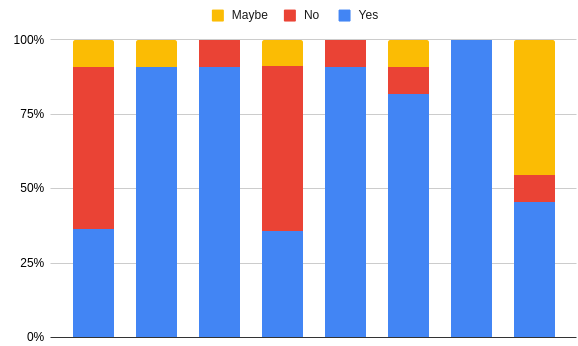
\includegraphics[width=\textwidth]{section3/emails.png}
        \caption{Participants performance on the phishing emails in the evaluation}
        \label{fig:emails}
    \end{center}
\end{figure}

Participants perfomed well when the sender is not netflix domain (netflix.com). Obvious fake domains such as fakenetflix.com, netflx.com, tinyurl.is and phishing.com were caught by the user (Column 6, Column 7, Column 8).

\section{Game Time vs perfomance}
We wanted to check if participants spending more time to complete the game performs better. To compare participants' performance before and after the game, we compute the f1-score\footnote{\url{https://en.wikipedia.org/wiki/F-score}} of each participant separately.

\begin{figure}[!ht]
    \begin{center}

        \subfloat[Ignoring "Maybe"]{
            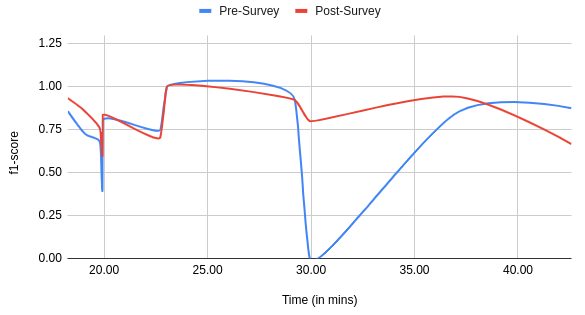
\includegraphics[width=0.9\textwidth]{section3/f1_without.png}
        } \\
        \hfill
        \subfloat[All emails]{
            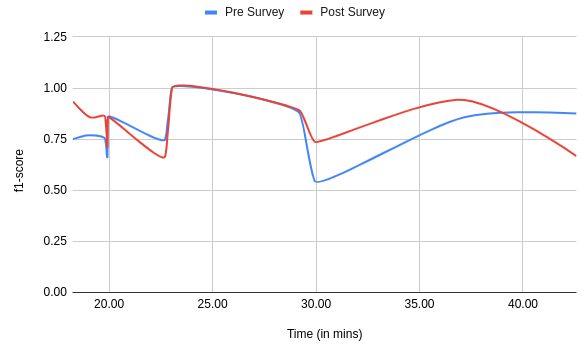
\includegraphics[width=0.9\textwidth]{section3/f1_with.png}
        }
        \hfill
        \caption{Comparison of f1-score before and after playing the game with time (Maybe answers are included)}
        \label{fig:f1_with_time}
    \end{center}

\end{figure}


Figure \ref{fig:f1_with_time} show f1-score of each participants with game time. Based on the chart, we can not conclude that higher game time results in better performance. However, we believe that with subtle hints and more emails, player playing longer will have better performance.

\section{Questionaire}
Table \ref{tab:game_questions} shows different opinion-based questions asked in the post-survey. The focus of the questionnaire was to assess participants' perceptions and opinions of the game and collect additional feedback about potential improvements.  Likert-scale questions used a 5-point scale ranging from 1 = strongly disagree to 5 = strongly agree.

\begin{table}[!ht]
    \centering
    \begin{tabular}{|r p{0.5\textwidth} r|}
        \hline
            & \textbf{Question}                                                                   & \textbf{Average Rating} \\
        1.  & The game showed phishing tricks.                                                    & 4.90                    \\
        2.  & I better understand phishing scams after playing the game.                          & 4.54                    \\
        3.  & I will use the techniques mentioned in the game to avoid phishing.                  & 3.9                     \\
        4.  & I understand spoofing better.                                                       & 4.18                    \\
        5.  & The game taught me how to protect myself from phishing.                             & 4.27                    \\
        6.  & I learned something new.                                                            & 4.72                    \\
        7.  & I know more about different link hiding techniques and what to look out for.        & 4.27                    \\
        \hline
        8.  & I would like to play the game again.                                                & 2.9                     \\
        9.  & The game is complicated.                                                            & 2.63                    \\
        10. & I prefer reading an educational document to playing a game to learn about phishing. & 1.81                    \\
        11. & Education games are important to understand security.                               & 4.45                    \\
        \hline
    \end{tabular}
    \caption[Likert scale questions relating opinion of the game]{Likert scale questions relating opinion of the game; Higher score means more positive response}
    \label{tab:game_questions}
\end{table}

Questions 1-7 (in table \ref{tab:game_questions}) focus on the educational features of the game and user feelings towards our approach. Based on the average score, we can see that participants welcomed the game and found it helpful. Figure \ref{fig:phishing_game_questions_1} summarizes the distribution of responses for each questions relating to phishing. We had positive responses for the game and techniques displayed in the game. For example, almost all participants agreed that the game showed phishing tricks and a majority of participants strongly agree that the game helped them understand phishing better.

\begin{figure}[!ht]
    \centering
    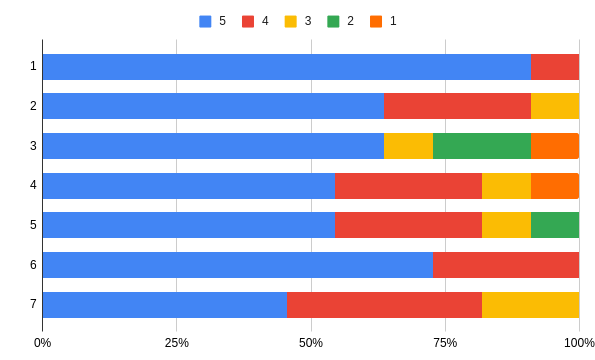
\includegraphics[width=0.8\textwidth]{section3/user_reponse_1.png}
    \caption[Responses to the first 7 questions]{Participants response to the first 7 questions. The numbers correspond to the question numbers in table \ref{tab:game_questions}.}
    \label{fig:phishing_game_questions_1}
\end{figure}

The second set of questions (8-11 in table \ref{tab:game_questions}) is related to participants' general opinions of the game and game-based learning. Figure \ref{fig:phishing_game_questions_2} illustrates the distribution of responses for question through 8-11.  More than half of the participants mentioned that they would not play the game again. We had a chance to talk to many of the participants and got common feedback on the gameplay. They were eager to play it the first time but would not like to play it again.

The majority of the participants did not find the game hard and could complete the game objective. However, we believe the game can be further simplified with better UI and hints to the player.

Finally, we asked participants their opinion on game-based learning. We can see that most of the participants prefer educational games over reading materials. Only one participant favored reading books over educational games for training purposes.


\begin{figure}[!ht]
    \centering
    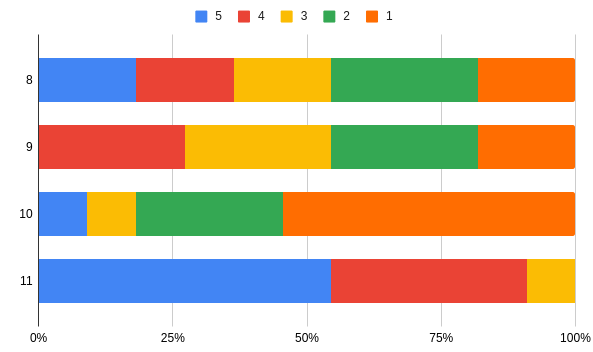
\includegraphics[width=0.8\textwidth]{section3/user_response_2.png}
    \caption[Responses to the 2nd set of questions]{Participants response to questions 8-11. The numbers correspond to the question numbers in table \ref{tab:game_questions}.}
    \label{fig:phishing_game_questions_2}
\end{figure}


\section{Participant Feedback}
At the end of the post-survey, we allow participants to express any comments or improvements to the game. The majority of the comments were positive about the game and pointed out it was a good experience. However, the majority of participants wanted a concise version of the game. One of the participants said he would ask his family to try out the game if it was short.

